
\section{Methodology}
\label{sec:methodology}

	In this section we outline our solution to our distributed state design. We discussion what protocols are used, how the clients and servers communicate and example game constructed for this system.
	
\subsection{The Client}

	The client locally simulates its own version of the game. To support this the client needs to keep a list of the other clients in the game and the most recent location of each client. This information will be stored in a map. At every simulation timestep in the game the client will send a position update to the server.
	
\subsection{The Server}

	The server simulates its own version of the game. The server is not used just to reduce message passing but also to act as an authority over the client to prevent cheating/malicious clients from propagating false information.
	
	In the simulation loop for the server a number of actions occur
	\begin{enumerate}
		\item The server's local copy of the clients locations are updated
		\item The server processes any events in its event queue
		\item If the events are valid the server is updated and the result is broadcast to the clients
	\end{enumerate}
	On a different thread
	\begin{enumerate}
		\item The server accepts position updates from clients
		\item The server verifies these updates to be valid
		\item The server broadcasts valid client updates
		\item the server accepts event messages and puts them in a queue for processing on the next timestep
	\end{enumerate}
	
	This way the server keeps the true state of the game and informs the clients of updates to the server's state. To perform these operations the server needs to have state for the currently active clients and its own version of the game state.

\subsection{The Game}

	We will simulate a very basic game to use as our state to synchronize. 
	The game has two possible actions \move{\agent}{\position} and \fire{\agent_{i}}{\agent_{j}}. These actions can be executed at any point in the game. 
	
	In order to simulate the game information is needed on the other agents in the game. The information needed for the game will be provided from the server or client the game is being simulated on. 
	
	\todo{Computer animations and therefore game simulations use simulation time. Simulation time can be used similar to a vector clock for synchronizing}
	
\subsection{Two Servers}

	In order to make the system more fault tolerant we can add another server to the \clientServer model. Having another server may provide more fault tolerance but a very difficult problem is introduced, server synchronization.
	
	\begin{figure}[ht]
		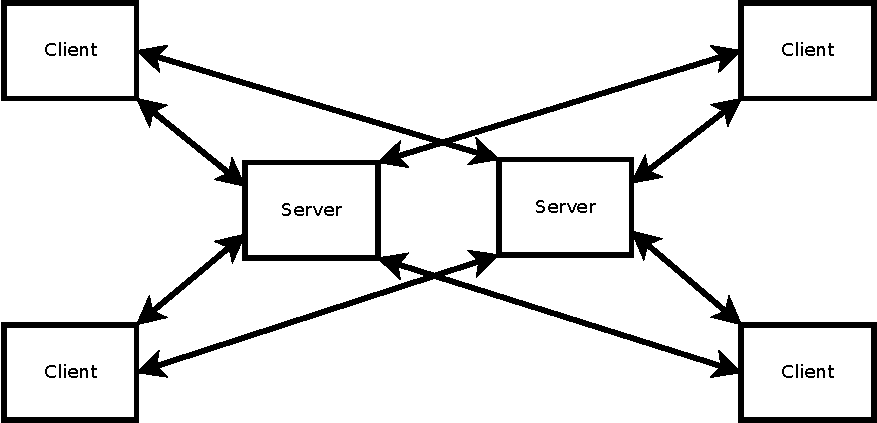
\includegraphics[width=0.95\linewidth]{../images/client-2server-model-crop.pdf}
		\caption{\label{figure:Client-2Server} \clientServer model with 2 servers.}
	\end{figure}
	
	The issue with this model is that there are definite server synchronization issues, this is due to the asynchronous message protocol. The asynchronous protocol leads to each server receiving messages in potentially different orders at potentially different times.
	
	We have thought of 3 different protocols to deal with this issue: (1) clients accepts the first response from a server, (2) clients accept the response with the smallest simulation time difference and (3) clients have a master server that they accept messages from. Each protocol has pros and cons, (1) can lead to conflict states by accepting messages from different servers. (2) This can induce lag into the system as the client waits for the best server response. (3) can still have issues when servers fail as a new master server will need to be chosen. We choose a combination of (2) and (3) and the reasons for this will be explained in section~\ref{subsec:distributed-servers}.
	
\subsection{Distributed Servers}
\label{subsec:distributed-servers}

	\todo{distributed server figure}

	\todo{Explain about changes to protocol and message passing between servers and clients}
		
\begin{comment}
		\begin{wrapfigure}{r}{0.20\textwidth} % controls margin around figure
		    \vspace{-28pt}
		  \begin{center}
		    \includegraphics[width=0.20\textwidth]{../images/cotan-diagram.pdf}
		    \vspace{-32pt}
		  \end{center}
	%		\setbeamerfont{figure:small-triangles}{size=\scriptsize}
		  \caption{\scriptsize\label{figure:small-triangles}2 adjacent triangles}
		\end{wrapfigure}
\end{comment}
	
\begin{comment}
\begin{enumerate}
	\item Common multiplayer model
		\begin{enumerate}
		\item latency minimization
		\item distributed state synchronization
		\item Avoiding cheating
	\end{enumerate}
	\item How Clients work
	\begin{enumerate}
		\item Client data
		\item Client messaging
	\end{enumerate}

	\item How the server works
	\begin{enumerate}
		\item Server data
		\item Server messaging
	\end{enumerate}
	\item The Game
	\begin{enumerate}
		\item The game keeps a natural vector clock (simulation time)
		\item Game data
		\item Game events/messaging
		\begin{enumerate}
			\item move
			\item fire
		\end{enumerate}
	\end{enumerate}
	\item Distributing the game
	\begin{enumerate}
		\item {Two server example}
		\item {Many server example}
		\begin{enumerate}
			\item The best serves can be choosen between two clients and most likely it will be the server on one of the two clients.
		\end{enumerate}
	\end{enumerate}
\end{enumerate}
\end{comment}
\todo{Up this point we have really only solved fault tolerance. If we want to solve some scalability issue we will need to provide spatial partitioning of the Game world.}

